\section{Durchführung}
\label{sec:durchführung}

\subsection{Aufbau}
\label{sec:aufbau}
Der Versuchsaufbau besteht aus einem PCB, auf welchem acht Thermoelemente $T1$ bis
$T8$ an drei Materialien Aluminium, Edelstahl und Messing angebracht sind. Die
Materialien werden von einem Peltierelement geheizt beziehungsweise gekühlt.
Der Betriebsmodus des Peltierelements kann über einen Schalter auf \textit{Heat}
oder \textit{Cool} geregelt werden. An das Peltierelement ist für die statische
Methode eine Spannung $U_P = 5 \si{\volt}$, für die dynamische Methode eine
Spannung von $U_P = 8 \si{\volt}$ angelegt. Die Daten der Thermoelemente werden
mithilfe eines Datenloggers \textit{Xplorer GLX} aufgenommen.
Der Versuchsaufbau ist in \ref{fig:aufbau} zu erkennen.

\begin{figure}[H]
  \centering
  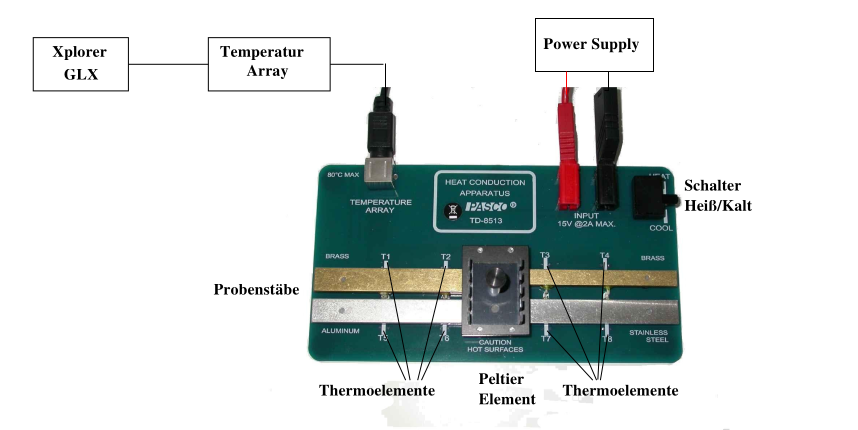
\includegraphics[scale=0.5]{pcb.png}
  \caption{Foto des Versuchsaufbaus.}
  \label{fig:aufbau}
\end{figure}
